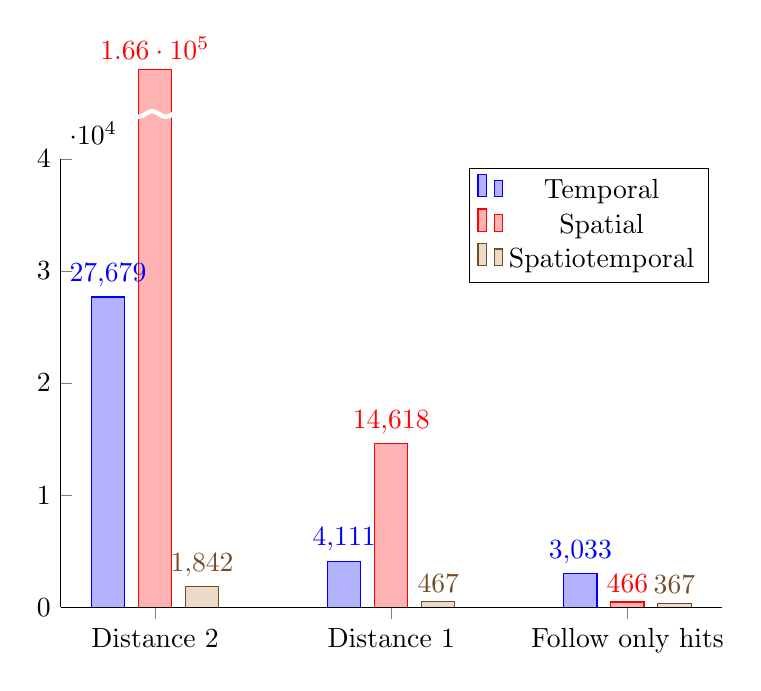
\begin{tikzpicture}
	\begin{axis}[
		title{Avg. time in ms}
		every axis plot post/.style={/pgf/number format/fixed},
		ybar=5pt,
		bar width=12pt,
		x=3cm,
		ymin=0,
		axis on top,
		ymax=40000,
		xtick=data,
		enlarge x limits=0.2,
		symbolic x coords={Distance 2, Distance 1, Follow only hits},
		restrict y to domain*=0:48000, % Cut values off
		visualization depends on=rawy\as\rawy, % Save the unclipped values
		after end axis/.code={ % Draw line indicating break
				\draw [ultra thick, white, decoration={snake, amplitude=1pt}, decorate] (rel axis cs:0,1.10) -- (rel axis cs:1,1.10);
			},
		nodes near coords={%
				\pgfmathprintnumber{\rawy}% Print unclipped values
			},
		axis lines*=left,
		clip=false,
		]
		\addplot coordinates {(Distance 2,27679) (Distance 1,4111) (Follow only hits,3033)};
		\addplot coordinates {(Distance 2,166479) (Distance 1,14618) (Follow only hits,466)};
		\addplot coordinates {(Distance 2,1842) (Distance 1,467) (Follow only hits,367)};
		\legend{Temporal, Spatial, Spatiotemporal}
	\end{axis}
\end{tikzpicture}